\section{Results}
\label{results}

\subsection{Ex-post structure: one natural split}
\label{sec:res-expost}

The data contain one clear division. In the Ward dendrogram the merge that joins the last two clusters is far higher than any other: 105.9, against 60.7 for the next merge and 42.0 for the one after. All three internal indices prefer $k=2$ for both algorithms (Table~\ref{tab:expost}, Figure~\ref{fig:expost}a). Beyond two clusters the indices flatten, with no second natural number of groups.

The two-cluster solution separates 932 small, quickly settled claims from the remaining 2,731:
\begin{itemize}[leftmargin=*]
\item \emph{small, fast claims:} median size 8,500, settled in a median of 1.5 quarters with 2 payments;
\item \emph{all other claims:} median size 125,000, settled in a median of 10.6 quarters with 5 payments.
\end{itemize}
Eighty-three per cent of the first group are below 20,000, so this is the short-delay band identified in Section~\ref{sec:dependence}. It accounts for only 1.9\% of total claim cost.

\begin{table}[!htbp]
\centering
\small
\caption{Ex-post clustering of the 3,663 claims: internal diagnostics and bootstrap stability. Silhouette and Calinski--Harabasz (CH): higher is better; Davies--Bouldin (DB): lower is better. Stability is the mean adjusted Rand index (ARI) over 20 bootstrap refits.}
\label{tab:expost}
\begin{tabular}{@{}lrrrrrrrr@{}}
\toprule
 & \multicolumn{4}{c}{K-means} & \multicolumn{4}{c}{Ward} \\
\cmidrule(lr){2-5}\cmidrule(l){6-9}
$k$ & Silh. & CH & DB & Stability & Silh. & CH & DB & Stability \\
\midrule
2 & 0.40 & 2,563 & 1.00 & 0.96 & 0.34 & 2,272 & 1.17 & 0.49 \\
3 & 0.27 & 2,128 & 1.29 & 0.94 & 0.26 & 1,895 & 1.20 & 0.51 \\
4 & 0.25 & 1,911 & 1.19 & 0.80 & 0.20 & 1,609 & 1.55 & 0.41 \\
5 & 0.25 & 1,748 & 1.25 & 0.79 & 0.20 & 1,490 & 1.35 & 0.41 \\
\bottomrule
\end{tabular}
\end{table}

\begin{figure}[!htbp]
\centering
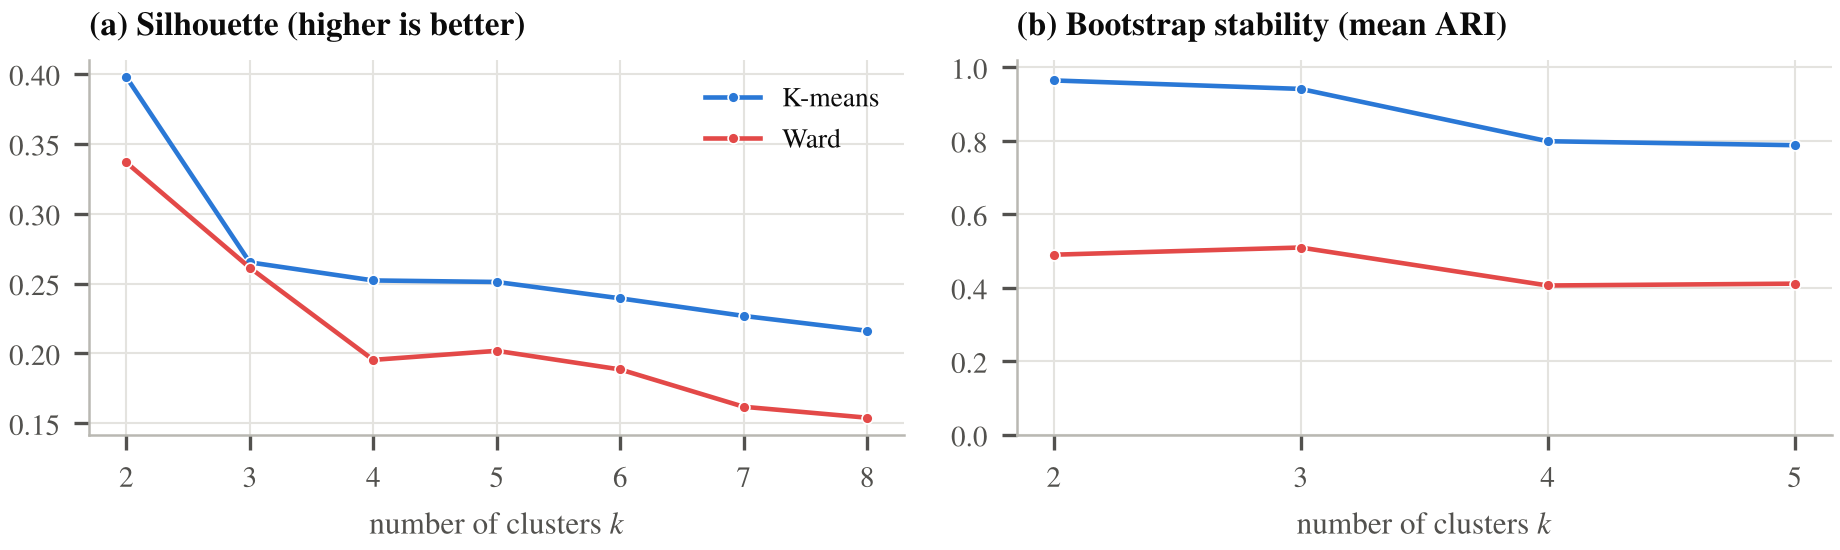
\includegraphics[width=0.95\textwidth]{fig_expost.png}
\caption{Ex-post clustering by number of clusters: (a) silhouette; (b) bootstrap stability (mean ARI between bootstrap and full-data partitions).}
\label{fig:expost}
\end{figure}

\emph{K-means is preferable to Ward on these data.} It scores better on every index at almost every $k$. It is also far more stable: its bootstrap ARI is 0.96 at $k=2$ and 0.94 at $k=3$, against about 0.5 for Ward at every $k$. Ward's greedy merges are never undone, so a change in a few early merges propagates to the final partition. The two algorithms agree only moderately (ARI 0.59 at $k=2$, 0.33--0.50 above).

\emph{Beyond two clusters, the partition reflects modelling choices more than structure.} Removing one of the three correlated complexity variables changes the K-means partition substantially (ARI against the baseline 0.52--0.74 for $k = 2,3,4$). Replacing them by a single complexity index, or decorrelating all four features, changes it more (ARI 0.26--0.61). By contrast, removing the largest 1\% of claims leaves the partition almost unchanged (ARI $\ge 0.97$).

At $k=4$ the groups are interpretable:
\begin{itemize}[leftmargin=*]
\item very small, fast claims (581 claims, 0.5\% of cost);
\item large, long-tailed claims with many payments (1,180 claims, 69\% of cost; median settlement delay 16 quarters, 7 payments);
\item two mid-size groups that differ mainly in notification delay (median 3.3 against 1.0 quarters).
\end{itemize}
The mix of these groups is stable across occurrence periods. Which finer partition is ``right'', however, depends on how much weight complexity should receive, and that is an actuarial judgement rather than a property of the data.

\emph{Practical implication.} Clustering finds the obvious split between small fast claims and the rest without supervision. Finer segments need an explicit justification for the feature weights, and should be reported together with their sensitivity.

\subsection{Experiment 1: segmenting the chain ladder}
\label{sec:res-cl}

At $\tau = 40$ the standard portfolio has:
\begin{itemize}[leftmargin=*]
\item 3,462 reported claims, of which 821 are open, and 201 IBNR claims;
\item 645 million paid to date;
\item actual RBNS run-off of 386.5 million;
\item outstanding case estimates of 252.5 million, 35\% short.
\end{itemize}
The shortfall of the case estimates is remarkably steady, between 34\% and 45\% at every valuation date in both portfolios.

\begin{table}[!htbp]
\centering
\small
\caption{Paid chain ladder RBNS reserve error by segmentation: mean absolute total error over six valuation dates ($\tau = 20,\dots,40$), and total error at $\tau = 40$. Clusters use features at notification; $k=3$ unless stated.}
\label{tab:cl}
\begin{tabular}{@{}lrrrr@{}}
\toprule
 & \multicolumn{2}{c}{Mean $|$error$|$ (\%)} & \multicolumn{2}{c}{Error at $\tau=40$ (\%)} \\
\cmidrule(lr){2-3}\cmidrule(l){4-5}
Method & Standard & Covariates & Standard & Covariates \\
\midrule
Unsegmented chain ladder & 31.8 & 21.2 & 35.0 & 28.3 \\
K-means, notification features & 33.6 & 22.7 & 34.0 & 30.8 \\
K-means, notification features, $k=4$ & 30.6 & 21.4 & 34.9 & 28.9 \\
Ward, notification features & 30.5 & 20.7 & 35.3 & 29.3 \\
K-means, notification features + covariates & -- & 23.0 & -- & 22.8 \\
True injury-severity groups & -- & 20.6 & -- & 22.7 \\
Bands of relative initial case estimate & 32.1 & 21.6 & 34.6 & 31.1 \\
Random groups, mean of 30 & 32.2 & 21.4 & 35.5 & 29.2 \\
\quad 5th--95th percentile at $\tau=40$ & & & 33.9--37.1 & 27.1--31.6 \\
Case estimates & 37.4 & 38.2 & $-34.7$ & $-37.4$ \\
\bottomrule
\end{tabular}
\end{table}

\begin{figure}[!htbp]
\centering
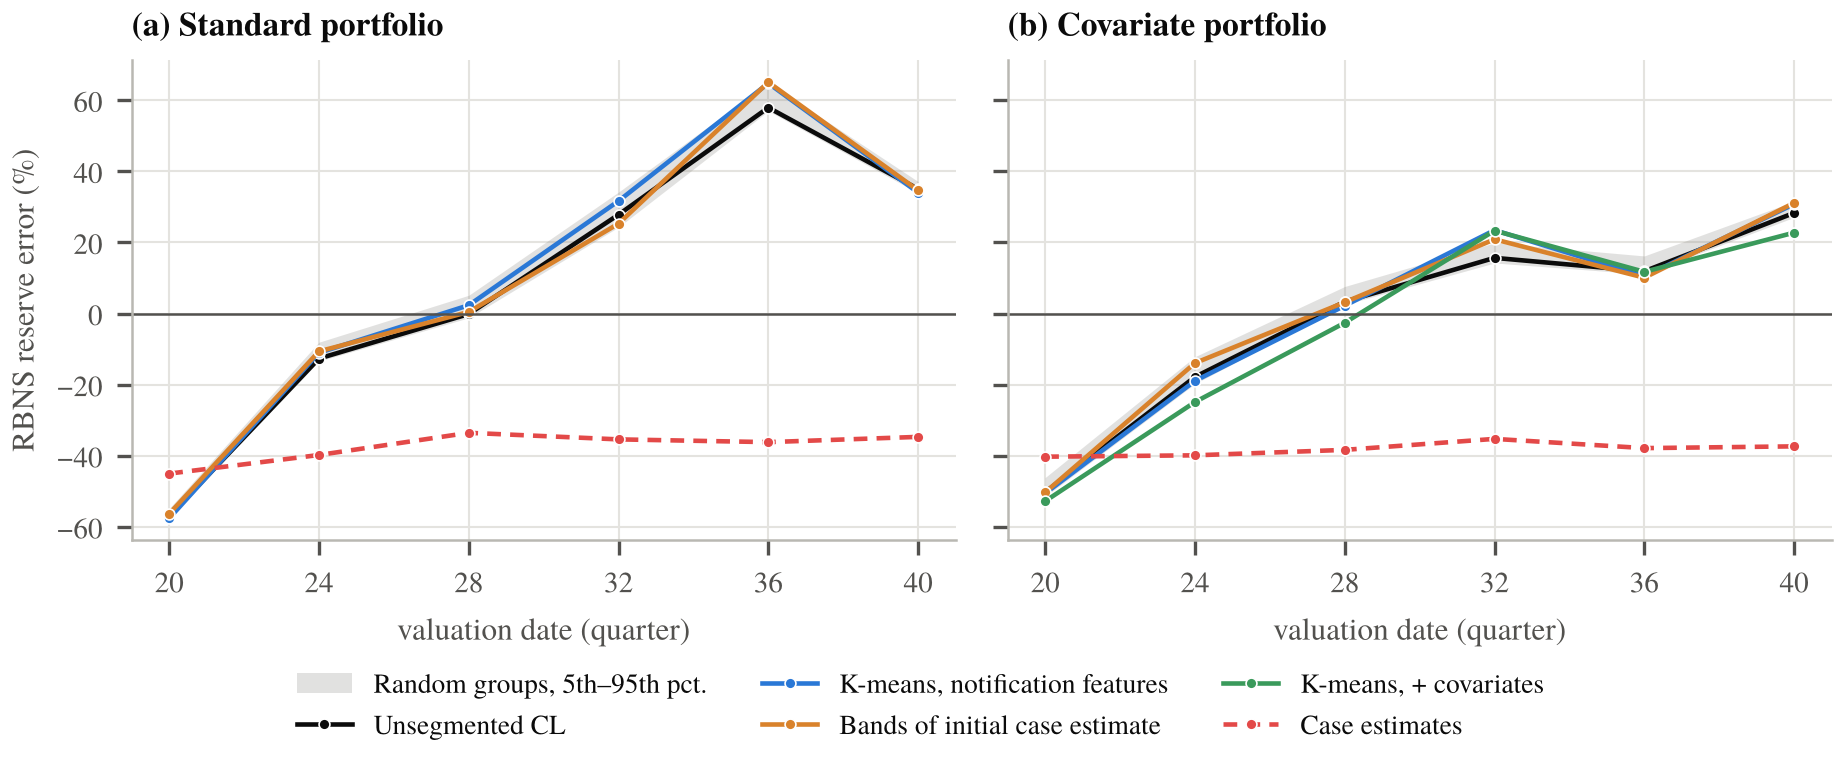
\includegraphics[width=0.95\textwidth]{fig_backtest.png}
\caption{RBNS reserve error of the paid chain ladder by valuation date, unsegmented and segmented. The shaded band is the 5th--95th percentile of 30 random segmentations with the cluster sizes.}
\label{fig:backtest}
\end{figure}

Table~\ref{tab:cl} and Figure~\ref{fig:backtest} show three things.

\emph{First, every method moves together over time.} Every segmentation underestimates by 45--59\% at $\tau=20$ and overestimates from $\tau=32$ onwards, by up to 80\% at $\tau=36$ in the standard portfolio.
\begin{itemize}[leftmargin=*]
\item The early underestimates reflect the missing tail: with only 20 notification periods, late development is not yet observed.
\item The later overestimates reflect two features of Complexity~5 that the chain ladder cannot accommodate: the steady acceleration of settlement over occurrence periods, and superimposed inflation.
\end{itemize}
Both are calendar-period effects, and no partition of claims removes them (Section~\ref{sec:segmentation}).

\emph{Second, segmenting by clusters gives no robust gain.} In both portfolios, clusterings on the notification features lie within a few points of the unsegmented chain ladder and of the random groups on average, and at $\tau=40$ inside the range of the random groups. The best method changes with $k$ and with the algorithm, which is what one expects of noise. The paid development patterns of the notification clusters are close to the aggregate pattern, so separate projection has little to correct. Banding the initial case estimate is no better.

\emph{Third, the covariates help at some dates but not on average.} At $\tau=40$, K-means with covariates and the true severity groups give $+22.8\%$ and $+22.7\%$, below the range of the random groups ($+27.1\%$ to $+31.6\%$). Over all six dates, however, the severity groups are only 0.6 points better than the unsegmented chain ladder (20.6\% against 21.2\%), and K-means with covariates is worse (23.0\%). A gain at a single valuation date is therefore not evidence of a useful segmentation, which is why we report the backtest over several dates.

\emph{Practical implication.} When the dominant source of error is a calendar-period effect, segmenting the triangle by claim type is unlikely to help. Any claimed gain should be compared with random segmentations of the same sizes.

\subsection{Experiment 2: adjusting case estimates}
\label{sec:res-oot}

The open claims at $\tau = 40$ show strong differences in case-estimate adequacy. A K-means grouping into four clusters on the valuation-date features separates them mainly by claim age:
\begin{itemize}[leftmargin=*]
\item \emph{just reported, nothing paid} (264 claims, median age 1.9 quarters): actual future payments are 2.65 times the case estimate;
\item \emph{mid-age claims} (308 claims, median age 7.9 quarters): a ratio of 1.48;
\item \emph{the two older groups} (249 claims): the case estimate is about right, with ratios of 0.97 and 1.01.
\end{itemize}
In-sample, the clusters together with the case estimate explain 45\% of the variance of log future payments, against 18\% for the case estimate alone.

Whether that difference can be exploited is a question for the out-of-time test (Table~\ref{tab:oot}, Figure~\ref{fig:oot}).

\begin{table}[!htbp]
\centering
\small
\caption{Out-of-time test: RBNS reserve error when factors \eqref{eq:lambda} fitted at $\tau_1 - 8$ are applied at $\tau_1$. Mean absolute total error over $\tau_1 = 24,\dots,40$, and median absolute log error per claim.}
\label{tab:oot}
\begin{tabular}{@{}lrrrr@{}}
\toprule
 & \multicolumn{2}{c}{Mean $|$error$|$ (\%)} & \multicolumn{2}{c}{Claim-level $|\log$ error$|$} \\
\cmidrule(lr){2-3}\cmidrule(l){4-5}
Method & Standard & Covariates & Standard & Covariates \\
\midrule
Raw case estimates & 35.9 & 37.7 & -- & -- \\
Unsegmented paid chain ladder & 26.7 & 15.4 & -- & -- \\
Single factor & 7.4 & 7.9 & 0.55 & 0.52 \\
Bands of claim age ($k=4$) & 6.3 & 7.8 & 0.61 & 0.59 \\
Bands of case estimate / initial estimate ($k=4$) & 3.5 & 8.6 & 0.64 & 0.64 \\
K-means clusters ($k=3$) & 4.9 & 8.3 & 0.66 & 0.64 \\
K-means clusters ($k=4$) & 5.2 & 8.0 & 0.68 & 0.63 \\
K-means clusters ($k=6$) & 5.7 & 7.8 & 0.51 & 0.63 \\
K-means clusters + covariates ($k=4$) & -- & 8.2 & -- & 0.63 \\
\bottomrule
\end{tabular}
\end{table}

\begin{figure}[!htbp]
\centering
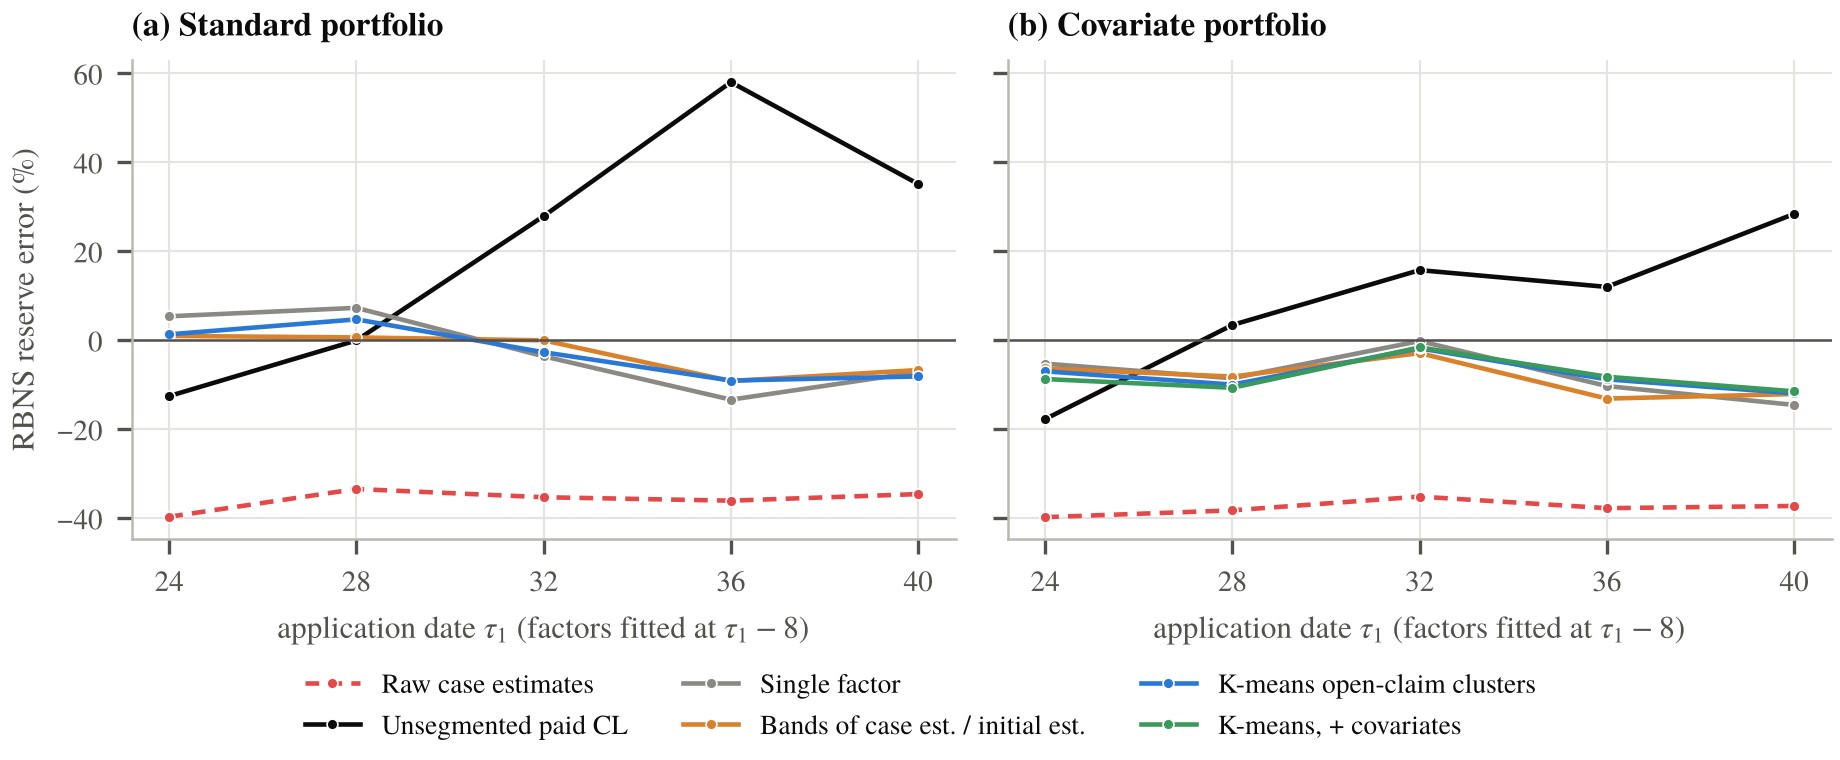
\includegraphics[width=0.95\textwidth]{fig_oot.png}
\caption{Out-of-time RBNS reserve error at the application date $\tau_1$, for case-estimate factors fitted eight quarters earlier, compared with raw case estimates and the unsegmented paid chain ladder.}
\label{fig:oot}
\end{figure}

\emph{Adjusting case estimates is far more effective than segmenting the triangle.} A single portfolio-wide factor, fitted eight quarters earlier, reduces the error from 36--38\% for raw case estimates to 7--8\%. That is better than the paid chain ladder in both portfolios, and the reason is the stability of the case-estimate shortfall noted above.

\emph{Grouping adds little.} In the standard portfolio, clusters with $k = 3$ or 4 reduce the mean error by 2.2--2.5 points relative to the single factor, but a simple rule does better: bands of the ratio of current to initial case estimate give 3.5\%. In the covariate portfolio no grouping improves on the single factor (7.8--8.6\% against 7.9\%), with or without the covariates. The clusters therefore add nothing over a rule an actuary could set by hand.

\emph{Groups improve the total, not individual claims.} The median absolute log error per claim is lowest for the single factor, or for six clusters in the standard portfolio, and no grouping improves it consistently.

All groupings drift negative at the later dates, to between $-6\%$ and $-13\%$ at $\tau_1 = 36$ and between $-2\%$ and $-15\%$ at $\tau_1 = 40$. This is the understatement built into \eqref{eq:lambda}, and it affects them all.

\subsection{Stability of the valuation-date clusters}
\label{sec:res-stability}

Expressing the initial case estimate relative to its notification period removes most of the drift. The largest change in cluster share between notification periods 1--20 and 21--40 falls from 11.5 to 3.8 percentage points in the standard portfolio, and from 11.8 to 3.6 points in the covariate portfolio. Bootstrap stability of the notification clusters rises from 0.70 to 0.96 at $k=3$ in the standard portfolio, and is 0.96 in the covariate portfolio.

Scale-free features matter for the open-claim clusters too. Clustering the open claims at $\tau=40$ on nominal amounts produces a group of 181 claims with small case estimates whose actual future payments are 9.9 times their case estimate. The group disappears with scale-free features, where the ratios range from 0.97 to 2.65 (Section~\ref{sec:res-oot}), so the extreme ratio depended on measuring amounts in nominal terms.

The groups that use the covariates are the least balanced. One open-claim cluster in the covariate portfolio contains only 14 claims, those without legal representation, which fails the credibility criterion even though it is stable.

\subsection{Experiment 3: other uses of groups, across the five scenarios}
\label{sec:res-uses}

Table~\ref{tab:scenarios} and Figure~\ref{fig:scenarios} report the mean absolute RBNS error over $\tau = 24,\dots,40$ for each method and scenario.

\begin{table}[!htbp]
\centering
\small
\caption{Mean absolute RBNS reserve error (\%) over $\tau = 24,\dots,40$, by method and SPLICE scenario (standard portfolios). Groups are K-means clusters on notification features ($k=3$), except the open-claim clusters ($k=4$).}
\label{tab:scenarios}
\begin{tabular}{@{}lrrrrrr@{}}
\toprule
Method & C1 & C2 & C3 & C4 & C5 & Mean \\
\midrule
Raw case estimates & 40.2 & 43.5 & 42.4 & 47.4 & 35.9 & 41.9 \\
\addlinespace
Paid chain ladder, unsegmented & 15.0 & 18.6 & 21.7 & 24.5 & 26.7 & 21.3 \\
Paid chain ladder by clusters & 16.9 & 19.4 & 21.1 & 24.1 & 28.8 & 22.1 \\
Paid chain ladder by random groups & 15.1 & 18.8 & 21.7 & 24.0 & 27.2 & 21.4 \\
\addlinespace
Case-estimate factor, single & 9.3 & 10.2 & 8.6 & 12.3 & 7.4 & 9.6 \\
Case-estimate factors, bands & 8.5 & 10.7 & 6.8 & 15.5 & 3.5 & 9.0 \\
Case-estimate factors, open-claim clusters & 8.7 & 10.6 & 8.2 & 14.2 & 5.2 & 9.4 \\
\addlinespace
Large claims apart, cluster & 10.6 & 8.8 & 10.7 & 9.4 & 14.3 & 10.8 \\
Large claims apart, rule & 9.2 & 11.2 & 10.2 & 9.1 & 13.4 & 10.6 \\
\addlinespace
GLM, no trend & 15.6 & 18.2 & 17.7 & 37.6 & 31.0 & 24.0 \\
GLM, calendar trend & 17.4 & 19.4 & 20.2 & 29.7 & 21.1 & 21.6 \\
GLM, calendar trend, by clusters & 17.7 & 19.4 & 21.3 & 27.2 & 23.0 & 21.7 \\
GLM, calendar and speed trends & 20.0 & 25.3 & 25.5 & 33.9 & 14.5 & 23.8 \\
GLM, calendar and speed trends, by clusters & 19.6 & 23.8 & 24.4 & 29.1 & 12.5 & 21.9 \\
\bottomrule
\end{tabular}
\end{table}

\begin{figure}[!htbp]
\centering
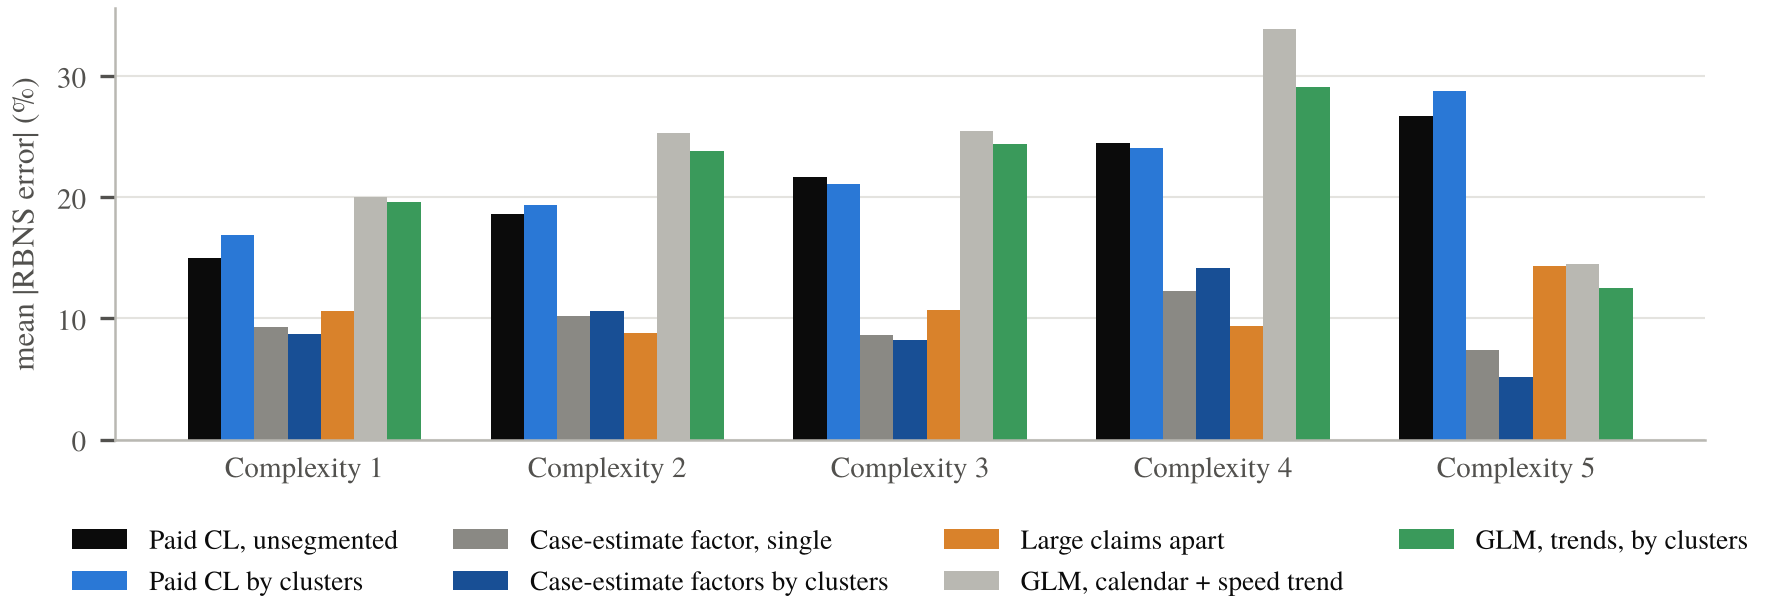
\includegraphics[width=0.95\textwidth]{fig_scenarios.png}
\caption{Mean absolute RBNS reserve error over $\tau = 24,\dots,40$ for the main methods, by SPLICE scenario.}
\label{fig:scenarios}
\end{figure}

\emph{Splitting the triangle fails in every scenario.} The clustered chain ladder is never better than the random groups. This includes Complexities~1 and~2, where no calendar-period trend can be blamed. The negative result of Section~\ref{sec:res-cl} is therefore not a feature of Complexity~5: in these simulations, the paid development patterns of the clusters are not different enough for separate projection to pay for the loss of data.

\emph{Adjusting case estimates is the most reliable approach.} A single factor gives 7--12\% in every scenario, and case-estimate factors are the best approach in Complexities~1, 3 and~5. Grouping does not improve it on average (9.4\% against 9.6\%), and simple bands do as well as clusters. The case estimates are short by 35--49\% at $\tau=40$ in every scenario, including Complexity~1, which has no inflation. The shortfall is therefore a property of how SPLICE generates case estimates, not an effect of inflation.

\emph{Treating large claims apart is the best approach when there is an inflation shock.} In Complexities~2 and~4 it gives the lowest errors, 8.8\% and 9.1--9.4\%. In Complexity~4 that is far better than the paid chain ladder (24.5\%) and the single case-estimate factor (12.3\%). It reduces the chain-ladder error in every scenario, by between 29\% (Complexity~1) and 62\% (Complexity~4). A threshold rule on the relative initial estimate defines the large group as well as the cluster does.

\emph{Groups add value inside a model that handles the calendar effects.} The calendar and speed trends help only where such trends exist. In Complexity~5 they reduce the GLM error from 31.0\% to 14.5\%. In Complexities~1--4 the speed trend extrapolates a pattern that is not there and increases the error. Within the model with both trends, however, group-specific development patterns reduce the error in every scenario (mean 21.9\% against 23.8\%; Complexity~4 29.1\% against 33.9\%; Complexity~5 12.5\% against 14.5\%). This is the one setting in which the clusters add value consistently: once the model accounts for the change over time, separating claim types refines it. The GLMs do not, however, beat the case-estimate factors in any scenario.

\emph{The groups make useful monitors} (Figure~\ref{fig:monitor}).
\begin{itemize}[leftmargin=*]
\item \emph{No false alarm without change.} In Complexity~1 no cluster shows a significant trend in settlement speed (Spearman $\rho$ 0.11--0.24, $p \ge 0.18$) or in its share of the portfolio.
\item \emph{A speed-up within the groups in Complexity~5.} Two of the three clusters settle significantly faster over time ($\rho = 0.51$, $p = 0.004$; $\rho = 0.42$, $p = 0.018$), and the share of the large cluster rises ($\rho = 0.60$, $p < 0.001$). The speed-up occurs within the groups, not only through the change in mix, which is why splitting the triangle cannot remove it.
\item \emph{Limited power with 30 cohorts.} In Complexity~3, where the speed-up is the designed feature, the signal is present in all three clusters but weak ($\rho$ 0.26--0.35, $p$ 0.06--0.16).
\end{itemize}

\begin{figure}[!htbp]
\centering
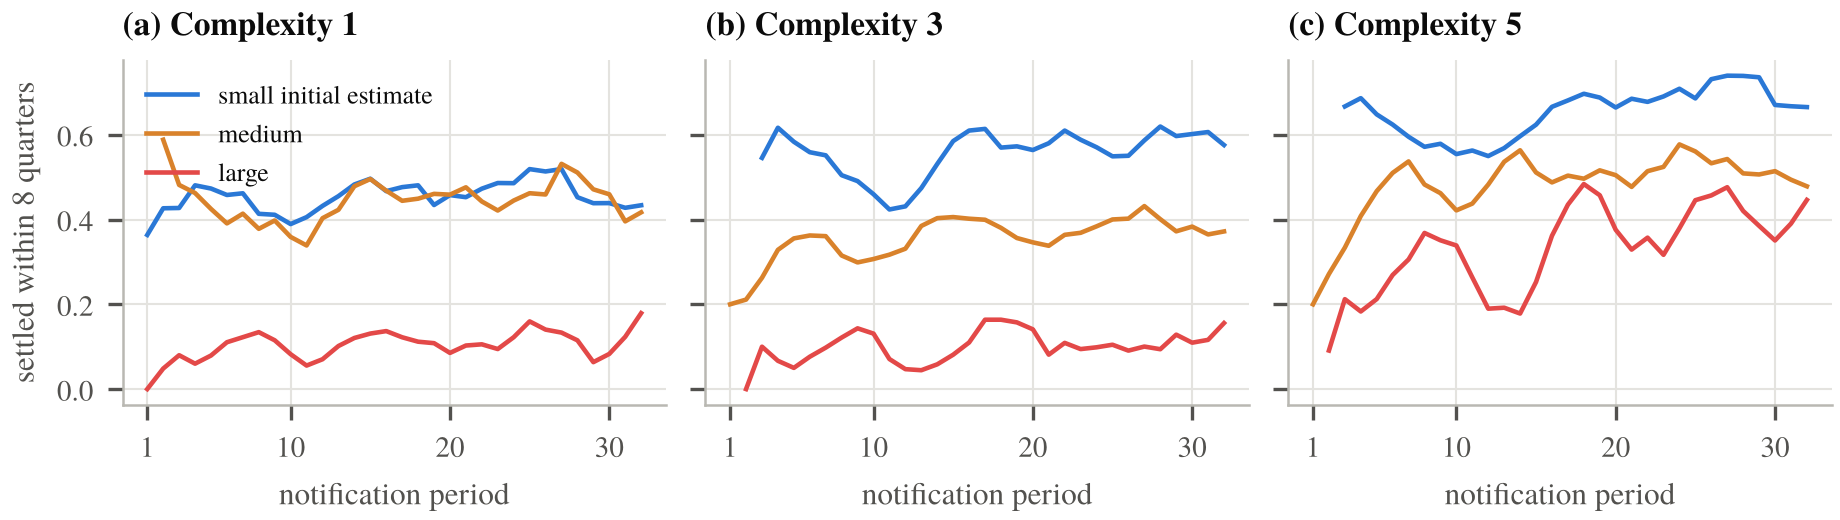
\includegraphics[width=0.95\textwidth]{fig_monitor.png}
\caption{Monitoring by cluster: share of claims settled within eight quarters of notification, by notification cohort (four-period moving average), at $\tau = 40$.}
\label{fig:monitor}
\end{figure}
